\documentclass[twocolumn]{revtex4}

\usepackage{graphicx}

\begin{document}

\title{
The Process of Predicting Weather
}

\author{Madison Taylor}
\affiliation{Siena College, Loudonville, NY}

\date{\today}

\begin{abstract}
	
	This article simulates the odds that it will rain on any given day in order to predict the estimated total amount of rainfall for a month. Predicting weather, more specifically rainfall, can be found through generating random numbers and looping them through a series of months to estimate a pretty accurate depiction of the odds it will rain. Throughout the six problems to solve in this Final Project, I have been asked, one,  to find the odds that it rains on one and only one day in a month, two, the odds that it rains at least eight days (in any order) that month, three, the odds that there are at least 10 cm of rain in a given month, and finally, to plot the distribution of rainfall as well as specify my confidence interval for the amount it will rain. Here I have provided a brief overview of my findings and predictions that will later be discussed more in depth. I have predicted that the odds it will rain on one and only one day given that there is a 20 percent chance it will rain on any day to be around 0.928 percent through an analytical approach and about 0.962 percent through my numerical approach (an approximate value due to the simulation utilizing random number generators). The chance it rains at least eight days (in any order) that month, given there is a 10 percent chance it will rain, I found to be approximately 0.767 percent and the odds that there are at least 10 cm of rain in a given month I found to be about 39.455 percent. Finally, I plotted my findings on a histogram to show the distribution of expected rainfall, found the average utilizing the odds I have found, and sorted my data to find that I am 95 percent confident that the rainfall will be between 0cm and 21cm. The article will provide further insight into my simulations and work throughout this project. 
	
\end{abstract}

\maketitle

\section{Introduction}
	The process of predicting weather is best solved using a Monte Carlo approach. Performing simulations that accurately calculate the chances that it will rain and the volume that it will rain, is necessary to further explain the fluctuating trends in weather. Weather, specifically rainfall in this project, is every changing. Throughout the Monte Carlo approaches described in this paper, weather can be analytically and numerically simulated to find the odds that it will rain for a given parameter, or amount of time, by generating random numbers and examining the probabilities of it actually raining. The goal here is to find these chances and ultimately predict the estimated amount of rainfall in a given month. 

\section{Problem 1}
	In problem 1 of predicting the weather, there is a 20 percent chance it will rain on any given day in a month. To analytically solve for the odds that it rains on one and only one day in a month, it is important to note that while on any day there is a 20 percent chance of rain, there is an 80 percent chance that it will in fact not rain. To better solve this problem, I am assuming that one month is equal to 30 days ($Days$) and keeping this logic consistent throughout the entirety of the project. 
	
	If the chances it will rain on any given day is 20 percent ($Prob_A$) and the chances it will not is 80 percent ($Prob_B$), I can easily identify the chances it will rain on one and only one day. Since I know the chance of it raining is 20 percent for one and only one day and 80 percent for the rest of the month (29 days). If I multiply these chances by 30, I can analytically solve for the answer during the whole month. To support this description is the equation and math below to further explain this analytical approach. 

$$(Prob_A*Prob_B^{Days-1})*Days$$
$$(.2*.8^{29})*30 = 0.00928 $$

	The calculation above depicts that the odds that it will rain on one and only one day of the month is 0.00928, which translates to 0.928 percent. 
	

\section{Problem 2}
	 In problem 2 of predicting the weather, we are supposing that there is a 10 percent chance that it will rain on any given day in a month. Numerically, I want to find the odds that it rains at least 8 days (in any order) that month. To work through this using a Monte Carlo Approach, I set a variable equal to the number of days (30) and a variable equal to the number of months (100,000) that I would like to use throughout my simulation. 
	 
	 The first step in approaching this problem was to define a function where I generate a random number between 0 and 1 and check to see if it is between between 0.0 and 0.10. If it is, then I set another variable to be True. The next step is to loop over the number of days in a nested loop over the number of months to check if any of the variables in my function were True. If they are, then I add the number one to another counter variable that I have defined. 

	Once the simulation has finished looping through the number of days, it takes the counter variable I have created and compares it to see if it is greater than or equal to 8. If it is, then I add number one to yet another counter variable that will count the number of months that has rained at least 8 days or more (in any order). In order to find the odds that it rains at least 8 days (in any order) that month using the simulation, the final step includes dividing the counter variable counting the number of months with 8 or more days by the number of months that the simulation looped over. 

\section{Problem 3a}
	In problem 3a of predicting the weather, I am trying to find the odds that there are at least 10 cm of rain in a given month. To solve this problem, it is necessary to understand the given facts of the problem, before approaching the simulation. 
	
	{\it~"Suppose that if it rains one day, the odds of a certain amount of rainfall on that day are 1 cm at 20 percent, 2 cm at 30 percent, 3 cm at 30 percent, 4 cm at 10 percent, and 5 cm at 10 percent. However the odds of it raining are dependent on if it rained the day before. If it is the first day of the month, there is a 10 percent chance of rain. If it rained 1 day before, but not 2 days before, there is a 20 percent chance of rain.  If it rained both of the 2 days before, but not the 3rd day before, there is a 25 percent chance of rain. If it rained for the 3 days (or more) before, there is a 5 percent chance of rain. Otherwise, there is a 10 percent chance of rain."}
	- Final Project Author and Master of CSIS 200
	
	For my simulation to solve for these odds, I first defined a function that will calculate the height in centimeters of how much it rained in one month. First I set a brand new variable counter equal to 0 and began to loop through the number of days provided for the function. In the loop I generate a random number between 0 and 1 and check to see if the random number falls within the 20 percent, 30 percent, or 10 percent parameters I defined. If the random numbers satisfy the argument range, then I have decided to add the respective number of centimeters it would have rained to the counter in this problem. 

	From here, I have looped through the number of months for each day in the month that there is at least 10 cm of rain in a given month. To do this, I first loop through the number of months, while setting the necessary counters needed to keep track of the total number of days it rained and the consecutive number of days that counts how many days in a row it rains. Using an array, I am able to add values that will keep track of days that it rained at least 10 cm and he days it did not.
	
	The final stages of this simulation is to add up the number of days in my array that were greater than or equal to 10 cm. Once that step is complete, I found the odds by dividing the total by the grand total number of months that I simulated. Finally, the probability of having 10 cm of rain in a given month is around 39 percent. 

\section{Problem 3b}
	The following histogram, see Figure \ref{Expected}, shows the distribution of expected rainfall values. Using the values from the Monte Carlo approach used in problem 3a, my simulation can be visually represented through this bell curve that is skewed to the right. This positive skew denotes that the mean is larger than the median.
	\begin{figure}[h]

		\centering
		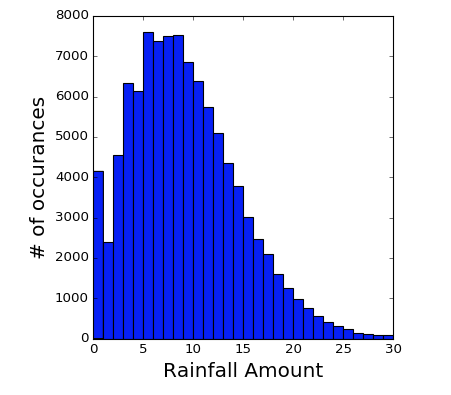
\includegraphics[width=0.5\textwidth]{rainfall.png}
		\caption{This is the distribution of expected rainfall values. \label{Expected}}

	\end{figure}

\section{Problem 3c}
	In problem 3c, calculating the average amount of rainfall in any given month is calculated using an array that I have defined earlier in the stages of problem 3a. Within the loop through the entire number of months (100,000) being tested, I created an array that would simply utilize the function I created to randomly add up the number of centimeters it rained. This array takes in the total number of days it rained and passes it through the function, to create an array containing the entire total of centimeters rained for each day in 100,000 months. Using pythons, numpy average function, I was able to easily generate the average expected rainfall to be about 8.67698 cm. 
	
\section{Problem 3d}
	In problem 3d of predicting the weather, I wanted to find the uncertainty (some people also refer to uncertainty as the "error") on my prediction. Using the sort function in python, I was able to copy my array, in order to reduce unnecessary changes, and sort it from the lowest to highest values. Since I am only concerned about the middle 95 percent, I found the lowest and highest 2.5 percent by multiplying the length of my array by .025. Using this value, i was able to cut off the bottom and top 2.5 percent of values in my array by indexing through the array for the middle 95 percent.
	Through these indices, I was able to find what rainfall is at the edge for the lower 2.5 percent and the higher 2.5 percent. Using the first index and the last index less one (to ensure it is the last value), I am now 95 percent confident that the rainfall will be between 0cm and 21 cm. 


\end{document}